\chapter{Complexity is Not a Curse: Leveraging Information in Interconnected Systems}
\label{chap_multiembed}

\section{Abstract}
Many real-world systems exhibit complex behaviors that result from interacting coupled components. This interconnectedness is often perceived as an obstacle for modeling, because of the difficulties in fitting mathematical equations with large numbers of variables. We present an alternative approach, Multiview Embedding (MVE), based on the concept of reconstructing system dynamics empirically from time series data. MVE uses the fact that each variable records not just its own behavior, but also that of interacting components, such that information is actually duplicated across different variables. By combining different models of the same system, forecasts can be dramatically improved, as we demonstrate for three model systems and a mesocosm experiment. Thus, MVE represents a new approach for information extraction, turning complexity into an advantage.

\section{Introduction}
A major challenge is to understand and predict complex systems, such as ecosystems, financial networks, and medicine. This is because much of the behavior in these systems is determined by interacting components, and even small perturbations of one variable can produce unexpected or catastrophic results on other parts of the system \cite{Scheffer_2001}. The study of these systems becomes especially difficult as complexity increases: more variables means a much greater increase in the number of possible interactions (the ``curse of dimensionality''; \cite{Donoho_2000, Fulton_2010}. Nevertheless, the ability to forecast these complex systems remains highly desirable, and would be of great utility in enabling targeted interventions or preemptive management actions to moderate the impacts of abrupt shifts \cite{Hill_2007, Doak_2008}.

Although traditional mathematical models have been applied to complex systems, they often show great sensitivity to parameters, model structure, and fitting routines \cite{Wood_1999}. Moreover, model complexity often exceeds what can be uniquely determined by the data. The alternative, strategically expedient, approach of reducing complexity (by e.g., aggregating species into trophic levels or functional groups, decomposing the system into independent components, holding parameters constant) can produce unrealistic behavior, leading to large uncertainties, overconfidence in long-term forecasts, and incorrect stability estimates \cite{Pahl-Wostl_1997, Fulton_2001, Clark_2001, Fulton_2003, Sugihara_2011}.

The identification of important interactions can itself be a challenging problem, with classical methods, such as correlation or Granger causality \cite{Granger_1969} insufficient when applied to systems with dynamic, state-dependent behavior \cite{Sugihara_2012}. Indeed, alternative frameworks that empirically reconstruct system behavior from data (Empirical Dynamic Modeling, EDM), have several advantages over classical approaches when modeling dynamic systems \cite{Perretti_2013, Deyle_2013, Ye_2015}. Here, we develop a new approach within the EDM framework to address the challenges associated with modeling high-dimensional complex systems.

\begin{figure}[!ht]
\begin{center}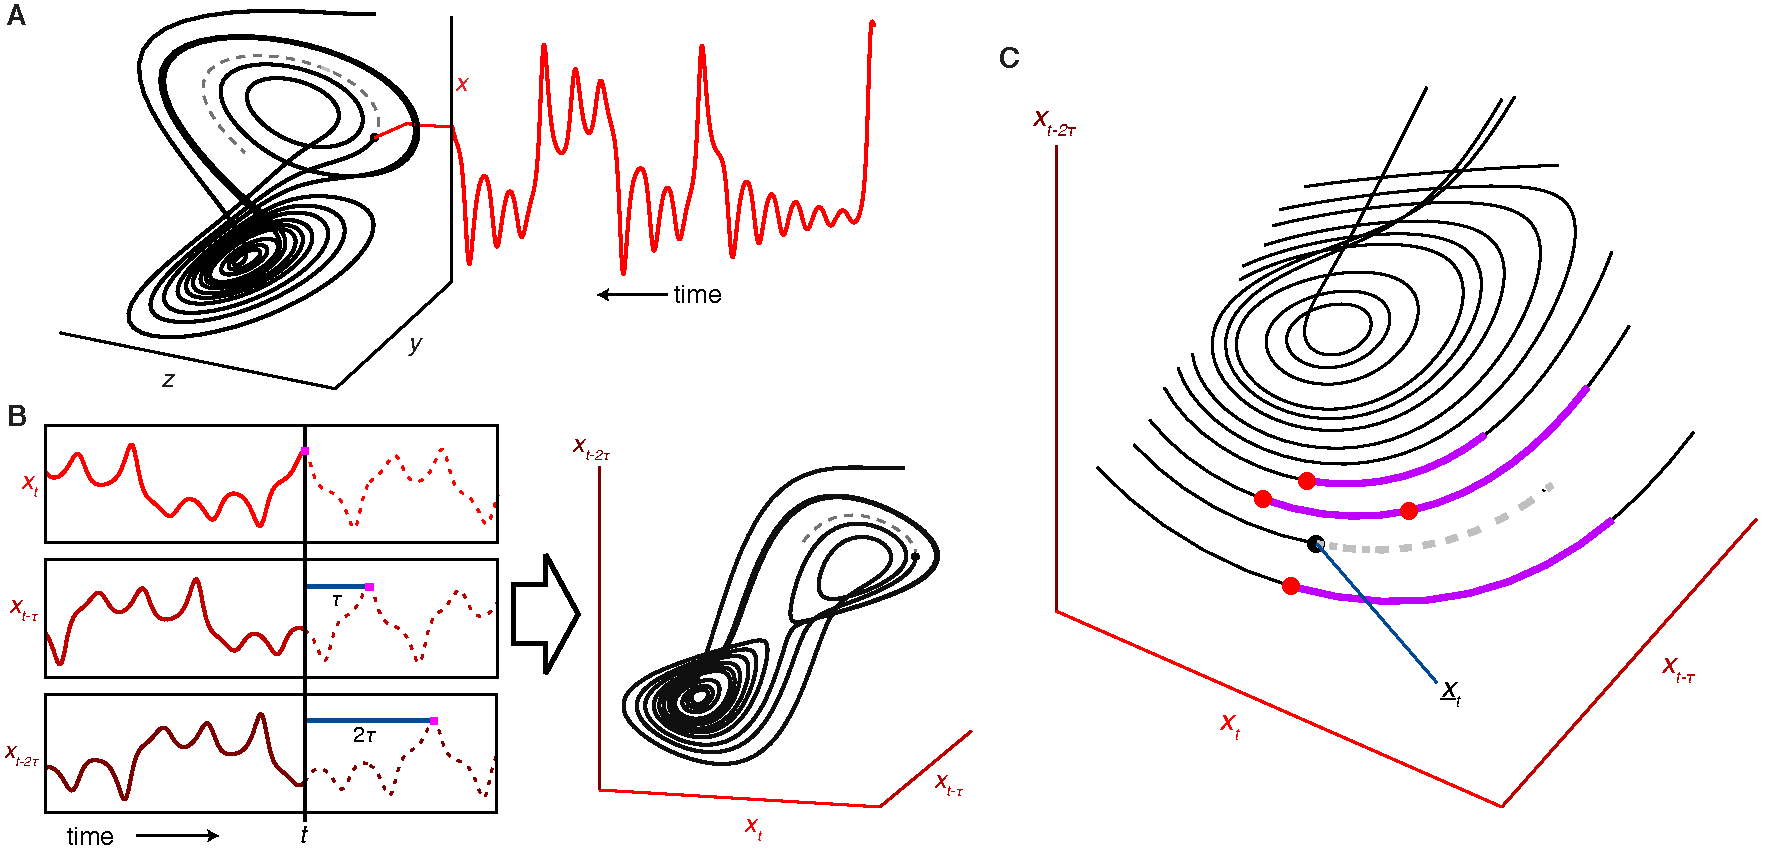
\includegraphics[width=\textwidth]{fig_multiembed_1.pdf}\end{center}
\caption[Attractor reconstruction from a time series.]{\textbf{Attractor reconstruction from a time series.}\newline
(A) Projecting the motion of the canonical Lorenz attractor onto the $x$-axis yields a time series for variable $x$. (B) Successive lags (with time step $\tau$) of the time series $x_t$ are plotted as separate coordinates to form a reconstructed ``shadow'' manifold, which appears similar to the original manifold in panel (A). (C) A magnified view shows nearest neighbor forecasting, whereby the nearest neighbors (red points) to the current observed vector $x_t$ (black point) are used to infer the behavior of the system going forward: the trajectories (purple lines) of the nearest neighbors are averaged to estimate the future behavior (gray dashed line) of $x_t$.}
\label{fig_multiembed_attractor_reconstruction}
\end{figure}

Unlike standard mathematical models, Empirical Dynamic Modeling (EDM) does not use hypothesized or assumed equations, and instead recovers behavior and interactions from the data directly. The essential idea is that time series are observations of the system dynamics (see Fig. \ref{fig_multiembed_attractor_reconstruction}a), which can be reconstructed by projecting successive lags of a single time series as separate coordinates (see Fig. \ref{fig_multiembed_attractor_reconstruction}b; \cite{Crutchfield_1979, Packard_1980, Takens_1981}). Using a sufficient number of lags, the dynamics unfold such that each point corresponds to a unique system state, with nearby points representing similar system states. These reconstructions can then produce forecasts via nearest-neighbor methods (see Fig. \ref{fig_multiembed_attractor_reconstruction}c; \cite{Lorenz_1969, Sugihara_1990}).

As a data-driven approach, EDM models are constrained by the available data: time series of 50 points or longer may be required to uniquely identify system states and nearest neighbors. This can be problematic for datasets that have been sampled for only short periods of time. One potential remedy is to combine data from multiple similar systems into a single composite attractor (``dewdrop regression'', \cite{Hsieh_2008, Clark_2015}) and increase the effective time series length. While reasonable in some situations, the requirement of dynamically equivalent time series is not always met, limiting the application of this technique. Moreover, while such methods directly address estimation error (i.e., an inaccurate model resulting from limited data), they do not address the issue of observational noise.

\begin{figure}[!ht]
\begin{center}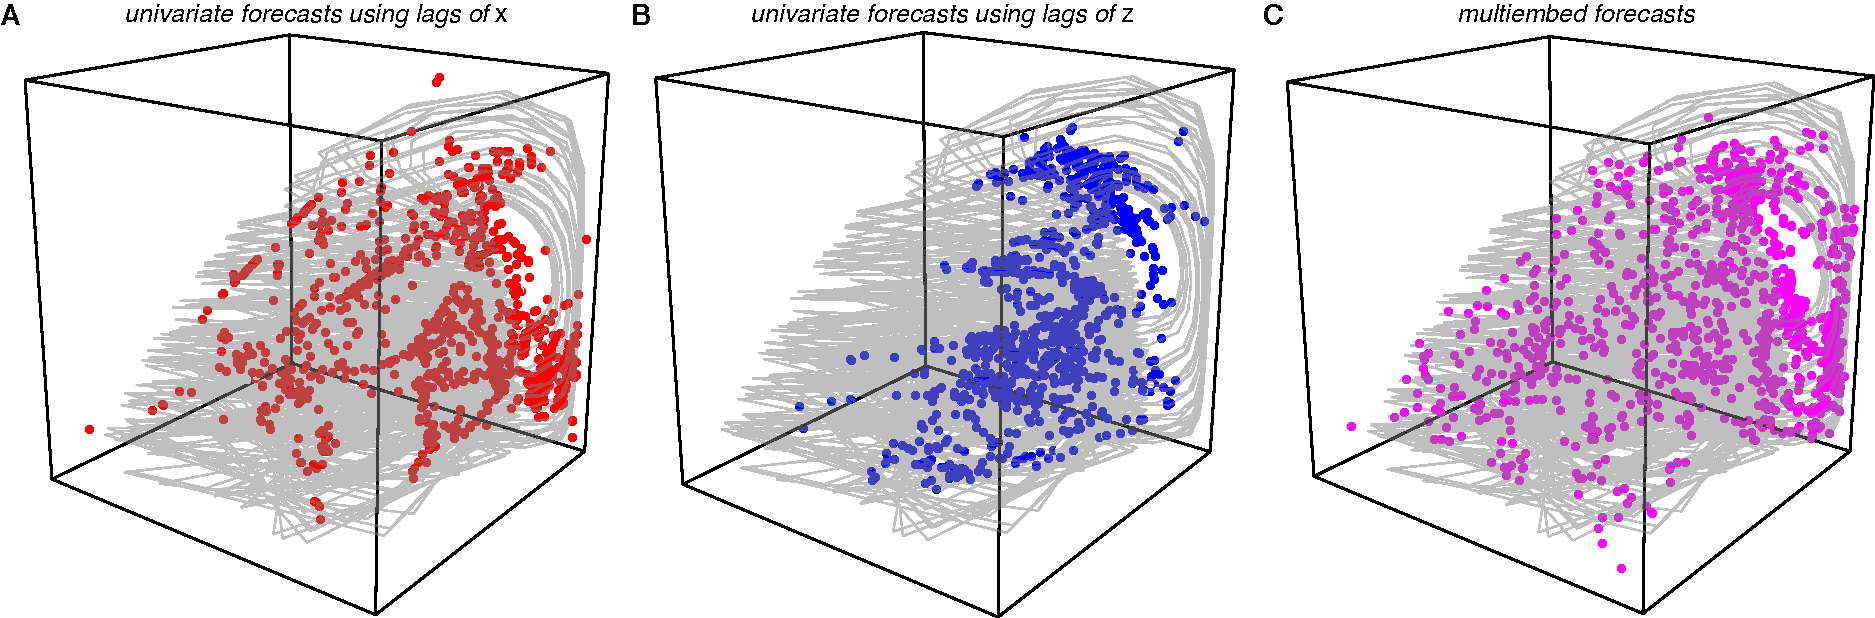
\includegraphics[width=\textwidth]{fig_multiembed_2.pdf}\end{center}
\caption[Information leverage in complex systems.]{\textbf{Information leverage in complex systems.}\newline
(A-B) Univariate reconstructions of the 3-species food chain model give incomplete views of the full system: predictions (solid points) only cover some portions of the original system attractor (grey lines) over the same time period. (C) Combining information from multiple reconstructions, the MVE model has a clearer depiction of the actual dynamics, resulting in predictions that span much more of the original system attractor. The same 1000 points are predicted by each model, based on the same 50 point library (see Methods).}\label{fig_multiembed_information_leverage}
\end{figure}

Here we introduce ``multiview embedding'' (MVE) as an EDM-based solution for modeling complex systems. The idea behind MVE is to exploit the property that time series contain information about causally related components \cite{Sugihara_2012}; as such, different time series from the same system contain redundant information. By combining these time series in different ways, multiple views of the same system can be constructed; together, these multiple then produce a clearer depiction of the dynamics (similar in spirit to stereoscopy where two 2D images form a single 3D image; see Fig. \ref{fig_multiembed_information_leverage}). In fact, because any generic combination of variables and lags is a valid reconstruction \cite{Sauer_1991, Deyle_2011}, the number of such views grows combinatorially with the number of variables, enabling substantial data leverage. Using $l$ lags for each of $n$ variables, the number of reconstructions of dimension $E$ is given by ${n l \choose E} - {n (l-1) \choose E}$\footnote{Note that ${n l \choose E}$ is the number of ways to choose $E$ coordinates from the $n l$ variable $\times$ lag combinations. The correction of ${n (l-1) \choose E}$ accounts for repeated counting (e.g., $\langle x(t), y(t) \rangle$ and $\langle x(t-1), y(t-1) \rangle$ represent the same reconstruction).}; with 10 time series, and $E = l = 3$, nearly 3000 different reconstructions are possible!

\section{Results}

\begin{figure}[!ht]
\begin{center}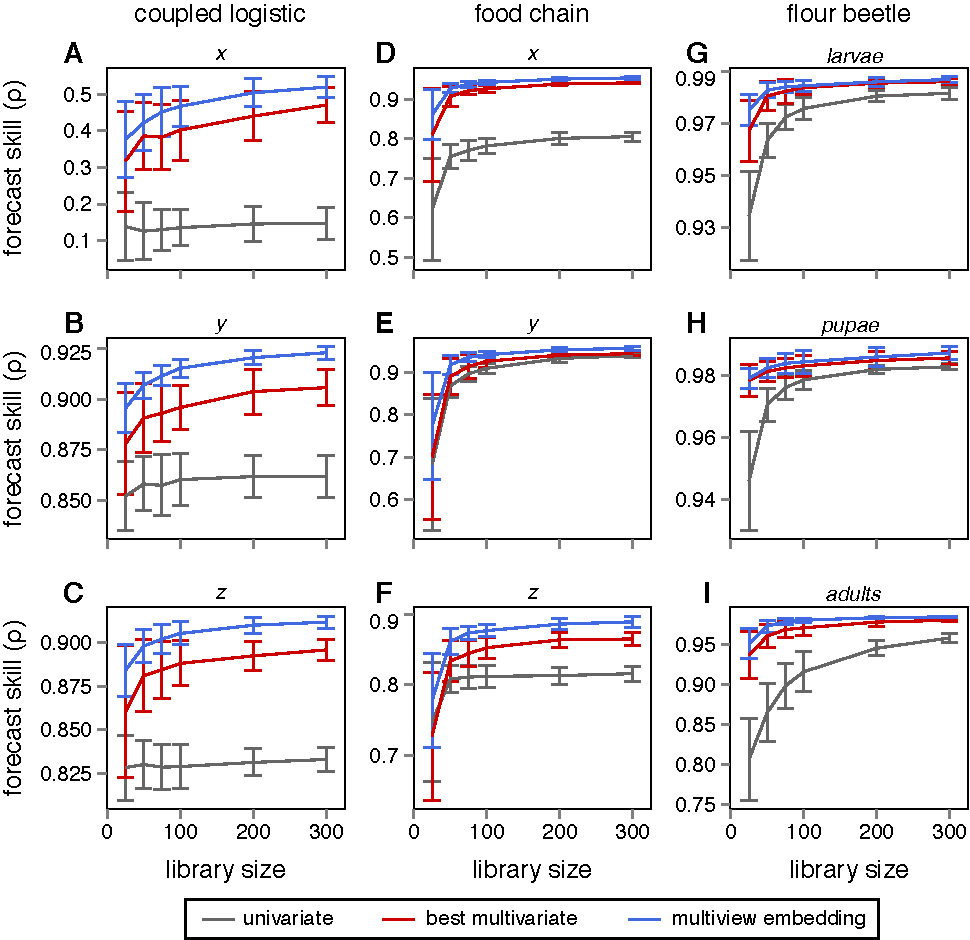
\includegraphics[width=\textwidth]{fig_multiembed_3.pdf}\end{center}
\caption[Comparison of forecast performance for model systems.]{\textbf{Comparison of forecast performance for model systems.}\newline
Multiview embedding produces more accurate forecasts than the best multivariate and univariate methods. (A-C) Forecast skill ($\rho$, correlation between observations and predictions) vs. library size for variables $x$, $y$, and $z$, in the coupled logistic map. Lines indicate average values over 100 randomly sampled libraries (see Methods) and error bars denote $\pm 1$ standard deviations. (D-F) Same as A-C, but for the 3-species food chain model. (G-I) Same as A-C, but for the flour beetle model.}
\label{fig_multiembed_model_results}
\end{figure}

To demonstrate multiview embedding (MVE), we implement a model-\linebreak averaging approach. First, we generate all possible reconstructions, computing the performance of each based on an in-sample training set (see Methods). Then, an MVE model is defined as the average of the top $25\%$ of these reconstructions and tested on an out-of-sample test set. Figure \ref{fig_multiembed_model_results} compares the performance of this MVE model with two commonly-used EDM methods: a ``univariate'' model, using only lags of the variable being forecast, and a ``best multivariate'' model, using the single reconstruction with the highest in-sample performance. For the three ecosystem models \cite{Hastings_1991, Dennis_2001}, MVE has the most predictive power (a measure of information gained; see Methods) as well as the highest accuracy ($\rho$, correlation between observations and predictions), and the lowest error (mean absolute error, MAE; and root mean square error, RMSE; see Figs. \ref{fig_multiembed_ed_1}-\ref{fig_multiembed_ed_3}).

\begin{figure}[!ht]
\begin{center}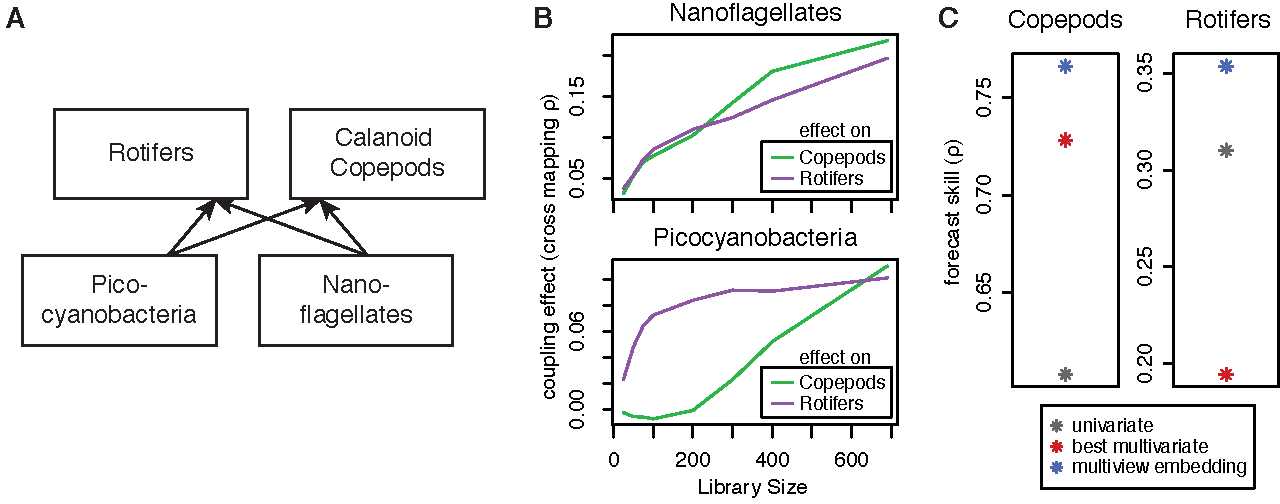
\includegraphics[width=\textwidth]{fig_multiembed_4.pdf}\end{center}
\caption[Analysis of the long-term mesocosm experiment.]{\textbf{Analysis of the long-term mesocosm experiment.}\newline
Panel (A) shows a portion of the food web. (B) Cross mapping between the grazers (calanoid copepods and rotifers) and the two prey items (nanoflagellates and picocyanobacteria) indicating causal influence of the prey items on the grazers. (C) Forecast accuracy ($\rho$) is higher for multiview embedding than for the univariate or best multivariate methods.}
\label{fig_multiembed_mesocosm_results}
\end{figure}

We next apply MVE to time series from a long-term mesocosm experiment \cite{Heerkloss_1998, Beninca_2009}. Here, convergent cross mapping \cite{Sugihara_2012} verifies that the two grazers (rotifers and calanoid copepods) are causally influenced by their prey (nanoflagellates and picocyanobacteria) (see Fig. \ref{fig_multiembed_mesocosm_results}ab). Thus, we produce models to forecast grazer abundances that include both prey time series as possible coordinates. Again comparing MVE to the ``univariate'' and ``best multivariate'' EDM models, the overall results are similar to those for the simulated ecosystems (see Fig. \ref{fig_multiembed_mesocosm_results}c, Fig. \ref{fig_multiembed_ed_4}), with MVE outperforming both of the other two methods.

\section{Discussion}
Accurate forecasts from a model require identification of the current state and estimation of how the system will evolve from that state. Consequently, predictive skill is diminished when a model does not clearly distinguish between states with divergent trajectories. Although Takens' Theorem and its generalizations suggest that all attractor reconstructions are valid \cite{Takens_1981, Sauer_1991, Deyle_2011}, in practical settings, observation error, limited time series length, and noise amplification mean that reconstructions can differ greatly in predictive skill \cite{Casdagli_1991}.

For example, in the 3-species coupled logistic map, forecasts produced by univariate models are inaccurate, and improve very little with more data (gray lines, Fig. \ref{fig_multiembed_model_results}a-c). This occurs because of the strong nonlinear interactions in this model: future values of a single variable, such as $y$, can depend greatly on the value of other variables ($x$ and $z$). In univariate models that include only lags of $y$, it can be difficult to infer the concurrent values of $x$ and $z$, thereby limiting forecast skill. Because of these limitations of univariate models, increasing the time series length may only result in marginal improvements in performance.

In contrast, multivariate models that include direct observations of the interacting variables can produce more complete depictions of the system dynamics.  The result is better forecasts that also show substantial improvement with increased library size (red lines, Fig. \ref{fig_multiembed_model_results}a-c). Because there are many ways to form multivariate reconstructions, we perform model selection on the in-sample data to choose the reconstruction that gives the highest accuracy. This enables the selection of the most relevant variables and lags for each forecast target. We further note that, unlike the traditional approach of creating a single complex model for the entire system, this model selection approach can select different reconstructions depending on the target variable. In other words, there is no single best model for the system, but a collection of different models for different components of the system.

Surprisingly, the MVE model produces better forecasts than the multivariate approach, even though MVE is essentially an average of different models (only one of which is the ``best'' multivariate model). We hypothesize that the improved performance of MVE is due to a reduced effect of observational error when combining multiple views of the system dynamics. Insofar as different time series variables can be reasonably assumed to have independent observation errors, combining different views of the system will increase precision and produce better forecasts. This is especially important when time series are short, because the reconstructions will be relatively sparse, and the selection of nearest neighbors will be unreliable. 

For example, in both the univariate and multivariate approaches, nearest neighbors are identified by distance in the reconstructed state space. If the data are subject to observation error, then the distance metric will be an uncertain measure of how similar these states actually are. Whereas points are normally weighted based on this distance metric, MVE effectively weights these points based on often it is the nearest neighbor among the best reconstructions. The improved forecasts suggest that this approach is a more reliable measure of whether points represent truly similar analogue states, thus allowing MVE forecasts to outperform single embedding-based models.

We note that noise reduction can also compensate for short time series length. For example, in the flour beetle model (see Fig. \ref{fig_multiembed_model_results}g-i), the dynamics appear to be well explained with the univariate method once time series are long enough ($\sim200$ points). However, in many practical circumstances, time series length is limited, and single reconstructions are not dense enough to counteract the effects of noise. Instead of requiring many neighbors to decrease error, MVE uses different reconstructions. Thus, at the smallest library size (25 points), the performance of MVE is often comparable to that of the best multivariate method with 2-3 times more data, and in many cases surpasses the univariate method even when the latter has 10 times more data.

Although we use a simple ranking and averaging scheme to implement MVE, more sophisticated methods to combine reconstructions (e.g., a weighted average, different ranking depending on system state) could produce further improvements, especially when larger datasets are available or when system-specific knowledge is available (e.g., noise structure, likely causal drivers). An obvious benefit to MVE is that with more time series, a clearer picture of the system dynamics emerges, as each additional variable increases the number of possible reconstructions. Because the number of reconstructions grows combinatorially with the number of variables, we suggest judiciously selecting only the relevant time series variables when applying MVE. As demonstrated here, convergent cross mapping (CCM) \cite{Sugihara_2012} can be used in conjunction with system-specific knowledge to identify the most informative variables for a given forecasting target. CCM is uniquely suited for this task, as it detects the presence of causal interactions using the same empirical framework as MVE.

\section{Conclusions}

The primary advantage of MVE is in leveraging multiple time series observations of a single system. That these time series represent interconnected components is actually a prerequisite for MVE, because it means that dynamical information is duplicated across different variables \cite{Sugihara_2012}. By using the equation-free approach of EDM, this information can then be extracted and re-combined. This approach to rich datasets allows MVE models to mitigate the effect of noisy observations, and is fundamentally different from other noise reduction algorithms.. For example, the Kalman filter \cite{Kalman_1960} assumes that the underlying dynamics are known and that noise is linearly separable, two assumptions that are typically unsuitable for complex systems.

Here, we demonstrate the usage of MVE to improve forecasts; however, MVE has potential benefits in many applications where noise reduction is a challenge, such as signal processing \cite{Carroll_2012} and nonlinear control systems \cite{Ott_1990}. Although the high-dimensionality of complex systems is typically perceived as an obstacle, MVE shows, counterintuitively, that complexity is actually an opportunity for information leverage.

\section{Methods Summary}

We used time series from 3 different models (a coupled logistic map, a 3-species food chain \cite{Hastings_1991}, and a flour beetle model \cite{Dennis_2001}) and data collected from a long-term mesocosm experiment (a plankton community isolated from the Baltic Sea; \cite{Heerkloss_1998, Beninca_2009}). For the model systems, 3000 points were generated with simulated observation error. For the mesocosm data, we sampled segments from the raw data, by using all segments of at least 15 points where the lag between points was 6-8 days, resulting in 17 segments comprising 725 data points. Time series were rescaled to mean = 0 and variance = 1.

For each model system, we generated all 3-dimensional attractor reconstructions, allowing lags of 0, 1, or 2, resulting in 64 unique reconstructions for each system. We applied a similar procedure to 2 subsystems from the mesocosm data, where each subsystem consisted of one of the grazers (rotifers or calanoid copepods) and its two main prey items (picocyanobacteria and nanoflagellates) (see Fig. 4a). We computed in-sample performance on ``library'' segments using simplex projection \cite{Sugihara_1990} and leave-one-out cross-validation to forecast 1 time step ahead. The attractors were then ranked based on $\rho$, the correlation coefficient between observations and predictions. This ranking identified the reconstructions to be used in the ``multivariate'' (best $\rho$) and MVE (top 16 $\rho$) methods when making out-of-sample forecasts.

We measured forecast skill using 4 different metrics: $\rho$, MAE (mean absolute error), RMSE (root mean square error), and predictive power (a measure of information gain \cite{Schneider_1999}). For the ecosystem models, we randomly subsampled 100 contiguous libraries (ranging in size from 25 to 300 vectors) from among the first 1300 points, and producing out-of-sample forecasts for the last 500 points. For the mesocosm data, we used an approximate 4-fold cross-validation scheme, assigning the 17 segments into 4 roughly-equally sized subsets.

\section{Methods}

\subsection{Data Sources}

We used time series generated from 3 different models (described below) and data collected from a long-term mesocosm experiment using a plankton community isolated from the Baltic Sea \cite{Hastings_1991, Dennis_2001, Heerkloss_1998, Beninca_2009}.

\subsection{Ecosystem Models}

\subsubsection{Coupled Logistic Map}

We modeled 3 interacting species using the coupled logistic map:

\begin{equation}
\label{eqn_coupled_map}
\begin{bmatrix}
x_{t+1}\\
y_{t+1}\\
z_{t+1} \end{bmatrix} = \vec{r} \circ 
\begin{bmatrix}
x_t\\
y_t\\
z_t \end{bmatrix} \circ 
\left(
\begin{bmatrix}
1\\
1\\
1 \end{bmatrix}
- A \times 
\begin{bmatrix}
x_t\\
y_t\\
z_t \end{bmatrix}
\right)
\end{equation}
where $\vec{r}$ is a $3 \times 1$ vector, $A$ is a $3 \times 3$ matrix with $A_{i, i} = 1$, and $\circ$ is the Schur product (entrywise product). We used initial conditions $\begin{bmatrix}
x_1\\
y_1\\
z_1 \end{bmatrix} = 
\begin{bmatrix}
0.2\\
0.2\\
0.2 \end{bmatrix}$, $r = \begin{bmatrix}
3.6\\
3.0\\
3.0 \end{bmatrix}$, and $A = \begin{bmatrix}
1 & 0.2 & 0.2\\
0.2 & 1 & -0.2\\
0.2 & -0.2 & 1 \end{bmatrix}$.

\subsubsection{3-species Food Chain}

We modeled a 3-species food chain following \cite{Hastings_1991}:

\begin{equation}
\label{eqn_3sp_food_chain}
\begin{array}{rl}
dx/dt &= x(1-x)-f_1(x)y\\
dy/dt &= f_1(x)y - f_2(y)z - d_1y\\
dz/dt &= f_2(y)z - d_2(z)
\end{array}
\end{equation}

where

\begin{equation*}
f_i(u) = a_i u / \left(1+b_i u \right)
\end{equation*}

We used the parameterization $a_1 = 2.5$, $b_1 = 3.2$, $b_2 = 2.0$, $d_1 = 0.2$, and $d_2 = 0.015$; and initial conditions $x_0 = 0.8$, $y_0 = 0.2$, and $z_0 = 8$.

\subsubsection{Flour Beetle Model}

We modeled 3 life stages (larvae, pupae, and adults) of the flour beetle, \emph{Tribolium castaneum} following \cite{Dennis_2001}:
\begin{equation}
\label{eqn_flour_beetle}
\begin{array}{rl}
L_{t+1} = b A_t \exp{\left(-c_\textrm{el}L_t - c_\text{ea}A_t\right)}\\
P_{t+1} = L_t \left(1 - \mu_l\right)\\
A_{t+1} = P_t \exp{\left(-c_\textrm{pa}A_t\right) + A_t\left(1 - \mu_a\right)}
\end{array}
\end{equation}
parameterization $b = 10.67$, $\mu_l = 0.1955$, $\mu_a = 0.96$, $c_\textrm{el} = 0.01647$, $c_\textrm{ea} = 0.01313$, and $c_\textrm{pa} = 0.35$, which are the maximum-likelihood estimates of the model parameters from real data, but with $c_\textrm{pa}$ adjusted to give chaotic dynamics \cite{Dennis_2001}. Initial conditions were $L_1 = 250$, $P_1 = 5$, and $A_1 = 100$.

\subsubsection{Time Series Generation}

The coupled logistic map and flour beetle model were run forward in time following equations \ref{eqn_coupled_map} and \ref{eqn_flour_beetle}, respectively. The 3-species food chain model was run by solving equation \ref{eqn_3sp_food_chain} using the classical Runge-Kutta method with a time step of 0.01 and downsampling by a factor of 800. For each model, we generated time series with 2000 points, and then simulated observation error by multiplying each time series with i.i.d. white noise drawn from a lognormal distribution with mean = 1 and CV (coefficient of variation) = 0.1. Next, we rescaled each time series to mean = 0 and variance = 1. (This ensures that the distance calculations for each attractor reconstruction are not skewed by the choice of coordinates.)

\subsection{Plankton Community}

This experiment has previously been described in numerous publications as an example of chaotic dynamics. We used the raw data from the supplement of \cite{Beninca_2009} and focused on forecasting the abundances of rotifers (mainly \emph{Brachionus plicatilis}) and the calanoid copepod \emph{Eurytemora affinis}. \cite{Beninca_2009} noted that the primary food items of the rotifers and calanoid copepods were picocyanobacteria and nanoflagellates (see Fig. \ref{fig_multiembed_mesocosm_results}a). We used convergent cross mapping \cite{Sugihara_2012} to verify that causal information about the prey abundances were present in the predator abundances (see Fig. \ref{fig_multiembed_mesocosm_results}b). Thus multivariate attractor reconstructions using the prey time series are suitable for forecasting the predators (rotifers and calanoid copepods).

Instead of interpolating the data (which can pollute the dynamics by combining information from multiple sampling times), we instead extracted all possible segments of 15 points or more and where the lag was 6-8 days ($\sim 1$ week). This procedure resulted in 17 segments, comprising 725 data points. Next, we applied the same fourth root transformation of \cite{Beninca_2009} to suppress sharp peaks that distort the attractor reconstruction (especially when searching for nearest neighbors) before applying the scaling procedure described above. Forecast statistics were computed after reversing the transformations.

\subsection{Attractor Reconstruction}

For each system, we generated all possible 3-dimensional attractor reconstructions where each coordinate could be any of the 3 time series variables with a lag of 0, $\tau$, or $2\tau$. Then we kept only the reconstructions where at least one coordinate had no lag, resulting in 64 attractors for each model system. For all models, we used $\tau = 1$. (Note that for the 3-species food chain model, $\tau$ is effectively 8, because we ran the model using a time step of 0.01 and downsampled by 800, and for the mesocosm data $\tau = 1$ corresponds to $\sim 1$ week.)

In the general case with $n$ time series variables, $l$ possible lags for each variable, and embedding dimension $E$, the number of possible attractor reconstructions is given by

\begin{equation*}
{n l \choose E} - {n (l-1) \choose E}
\end{equation*}

where ${n l \choose E}$ is the number of attractors formed by choosing $E$ of the $nl$ possible coordinates, and ${n (l-1) \choose E}$ is the number of ``invalid'' attractors where all $E$ coordinates are chosen from among the $n(l-1)$ possible coordinates with positive (i.e. nonzero) lag.

\subsection{Multiview Embedding}

Using the method of simplex projection \cite{Sugihara_1990} and leave-one-out cross-validation, we computed the performance of each attractor reconstruction when forecasting 1 time step ahead on an in-sample portion of the data, called the library. The attractors were ranked based on $\rho$, the correlation coefficient between observations and predictions. The top attractors were then used to produce forecasts for the out-of sample portion of the data. The multiview embedding forecast is defined to be the arithmetic mean of the forecasts from the top attractors:

\begin{equation*}
\hat{y}_{t+p} = \frac{1}{m} \sum_{i = 1}^{m}{y_{nn_1^i(t)+p}}
\end{equation*}

where $m$ is the number of attractors to average over (16 in this case), $nn_1^{i}(t)$ is the time index of the nearest neighbor in the $i$th attractor at time $t$, and $p = 1$ is the prediction horizon.

Conventional simplex projection \cite{Sugihara_1990} uses $b$ nearest neighbors from a single attractor reconstruction, and each of these neighbors represents a unique historical state. These neighbors are weighted by their distance, which is influenced by observational error, so forecasts can be quite sensitive to noise. However, multiview embedding uses the single nearest neighbor from $m$ attractor reconstructions. As these points potentially represent the same historical state and have different observation errors, averaging over them will give a larger weighting towards the points that are consistently closer to the actual system state, in a manner similar to the weighted average used in simplex projection.

\subsection{Performance Metrics}

Forecast skill was measured using 4 different metrics: $\rho$, the correlation coefficient between observations and predictions; MAE, mean absolute error; RMSE, root mean square error; and predictive power \cite{Schneider_1999}. $\rho$ captures forecast accuracy, how well the predictions line up with observations. Both MAE and RMSE capture forecast error, the ``average'' deviation of predictions from observations. Predictive power is an information-theoretic measure that indicates how much uncertainty in the predicted variable is reduced by forecasts.

For the model data, we sampled 100 libraries from the generated time series by choosing the beginning of each library from the uniform distribution [501, 2001]. (Note that we exclude the first 500 points from each time series, so as to reduce the effect of transient behavior.) Out-of-sample forecasts were then produced for last 500 points of the time series (times 2501-3000). The libraries ranged in size from 25 to 300 vectors ($L \in \{25, 50, 75, 100, 200, 300\}$); thus, there was no overlap between the library and forecasts, because the last possible point in the library is at time 2500 and the first point to be forecast is at time 2501. For the mesocosm data, we used a 4-fold cross-validation scheme where 1/4 of the data was held out of sample and the remaining 3/4 was the ``library''. The forecasts for each quarter of the data were then combined before computing statistics. (Note that although the statistics are computed once over the whole time series, the attractors were ranked separate for each 1/4 of the data, so that all forecasts are out-of-sample.).

\section{Extended Data Figures}

\begin{figure}[!ht]
\begin{center}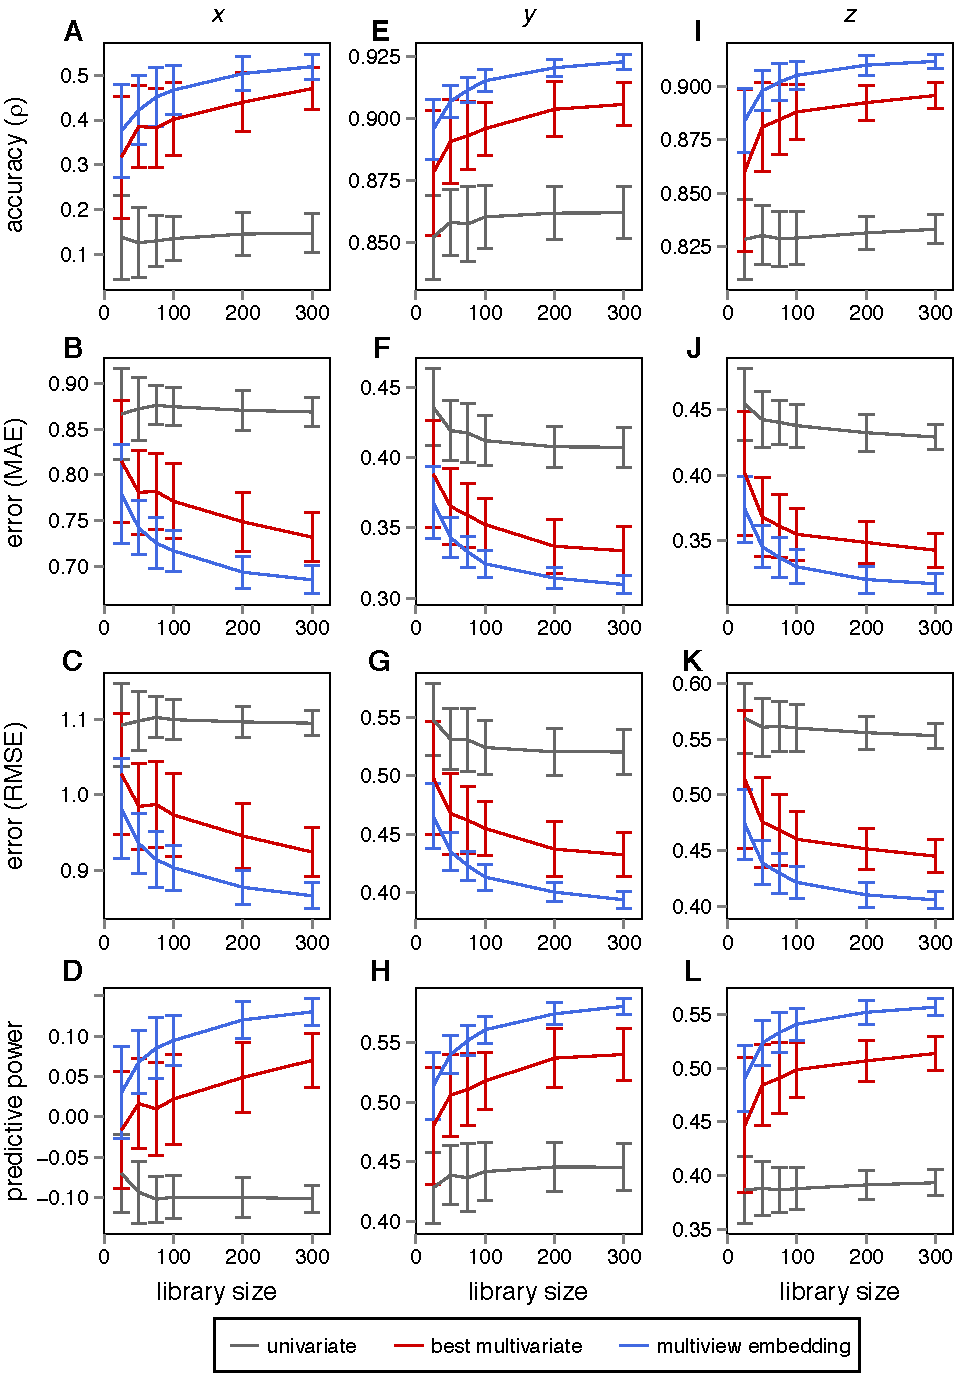
\includegraphics[scale = 0.65]{fig_multiembed_ed_1.pdf}\end{center}
\caption[Comparison of forecast performance for the 3-species coupled logistic map model.]{\textbf{Comparison of forecast performance for the 3-species coupled logistic map model.}\newline
Multiview embedding produces more precise forecasts than the best multivariate and univariate methods for the 3-species coupled logistic map model. (A-D) Forecast accuracy ($\rho$, correlation between observations and predictions), forecast errors (MAE, mean absolute error; RMSE, root mean square error), and predictive power vs. library size for variable $x$. Lines indicate average values over 100 randomly sampled libraries (see Methods) and error bars denote $\pm 1$ standard deviations. (E-H) Forecast accuracy, forecast errors, and predictive power for variable $y$. (I-L) Forecast accuracy, forecast errors, and predictive power for variable $z$.}
\label{fig_multiembed_ed_1}
\end{figure}

\begin{figure}[!ht]
\begin{center}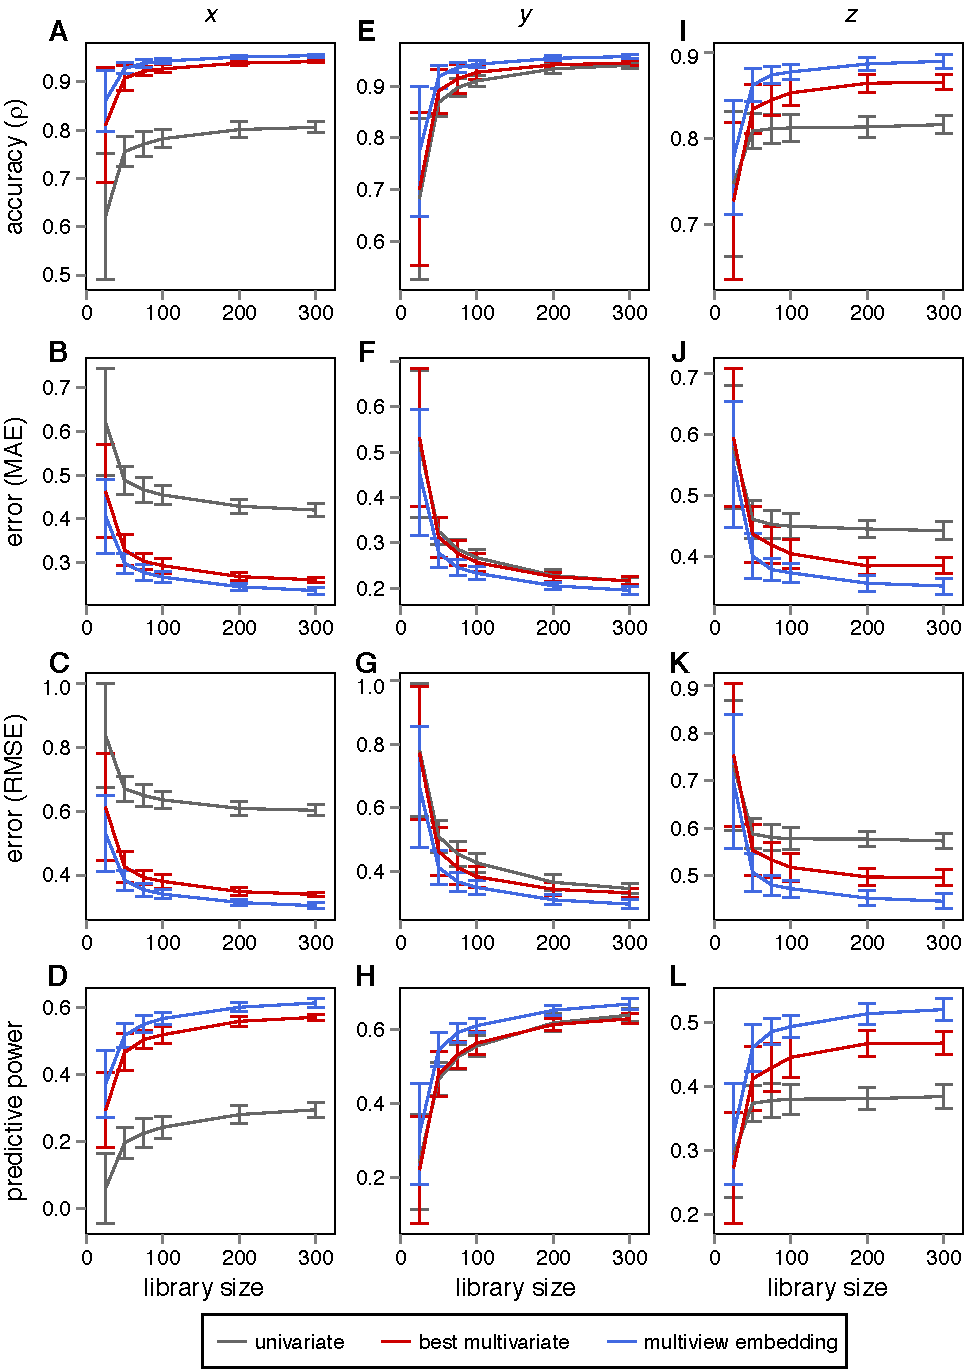
\includegraphics[scale = 0.65]{fig_multiembed_ed_2.pdf}\end{center}
\caption[Comparison of forecast performance for the 3-species food chain model.]{\textbf{Comparison of forecast performance for the 3-species food chain model.}\newline
Multiview embedding produces more precise forecasts than the best multivariate and univariate methods for the 3-species food chain model. (A-D) Forecast accuracy ($\rho$, correlation between observations and predictions), forecast errors (MAE, mean absolute error; RMSE, root mean square error), and predictive power vs. library size for variable $x$. Lines indicate average values over 100 randomly sampled libraries (see Methods) and error bars denote $\pm 1$ standard deviations. (E-H) Forecast accuracy, forecast errors, and predictive power for variable $y$. (I-L) Forecast accuracy, forecast errors, and predictive power for variable $z$.}
\label{fig_multiembed_ed_2}
\end{figure}

\begin{figure}[!ht]
\begin{center}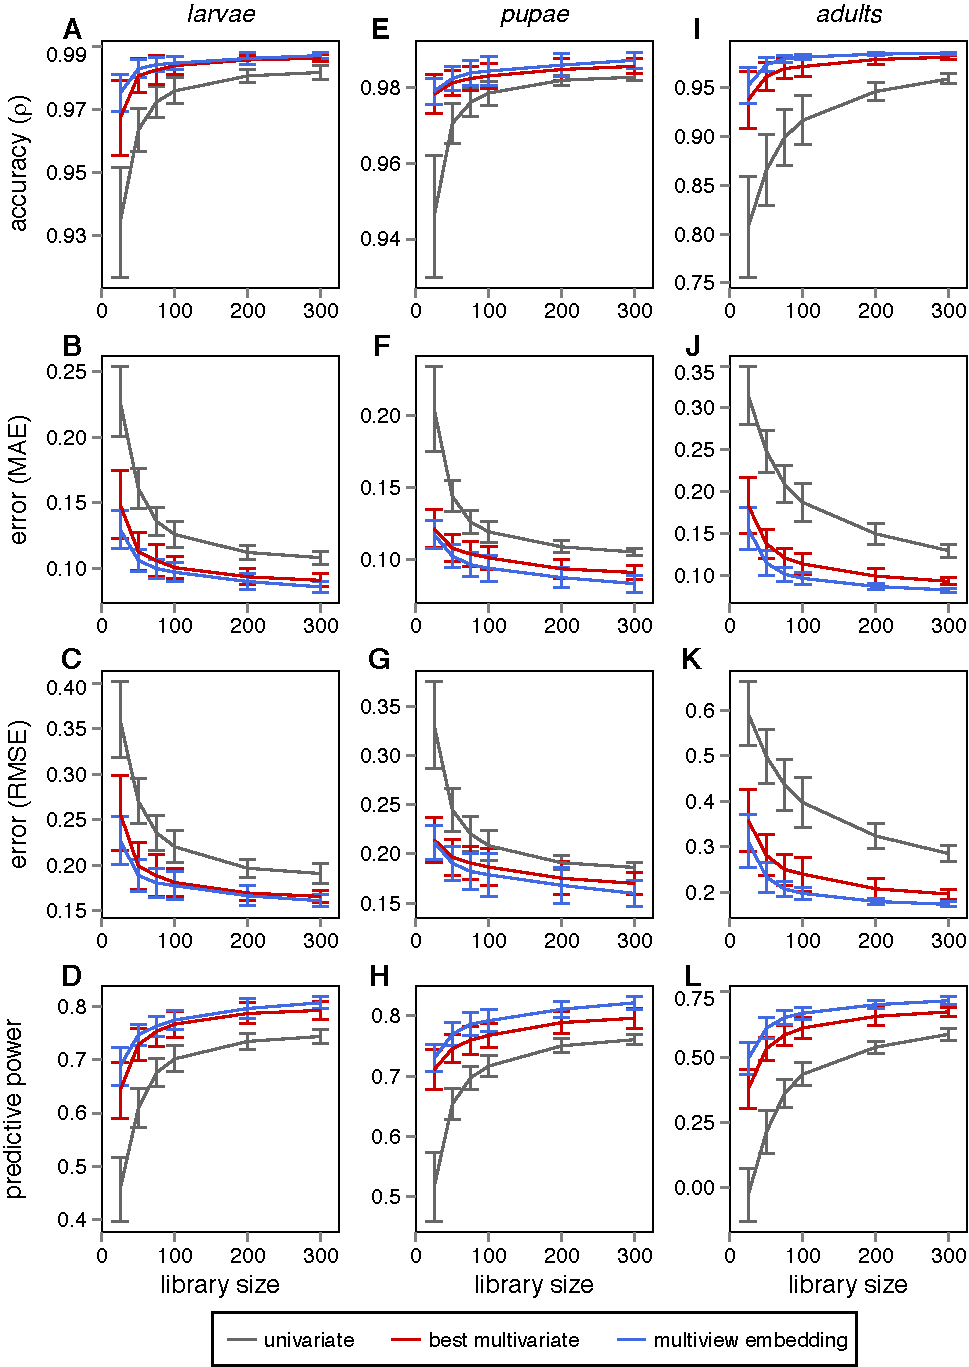
\includegraphics[scale = 0.65]{fig_multiembed_ed_3.pdf}\end{center}
\caption[Comparison of forecast performance for the larvae-pupae-adult flour beetle model.]{\textbf{Comparison of forecast performance for the larvae-pupae-adult flour beetle model.}\newline
Multiview embedding produces more precise forecasts than the best multivariate and univariate methods for the larvae-pupae-adult flour beetle model. (A-D) Forecast accuracy ($\rho$, correlation between observations and predictions), forecast errors (MAE, mean absolute error; RMSE, root mean square error), and predictive power vs. library size for larvae. Lines indicate average values over 100 randomly sampled libraries (see Methods) and error bars denote $\pm 1$ standard deviations. (E-H) Forecast accuracy, forecast errors, and predictive power for pupae. (I-L) Forecast accuracy, forecast errors, and predictive power for adults.}
\label{fig_multiembed_ed_3}
\end{figure}

\begin{figure}[!ht]
\begin{center}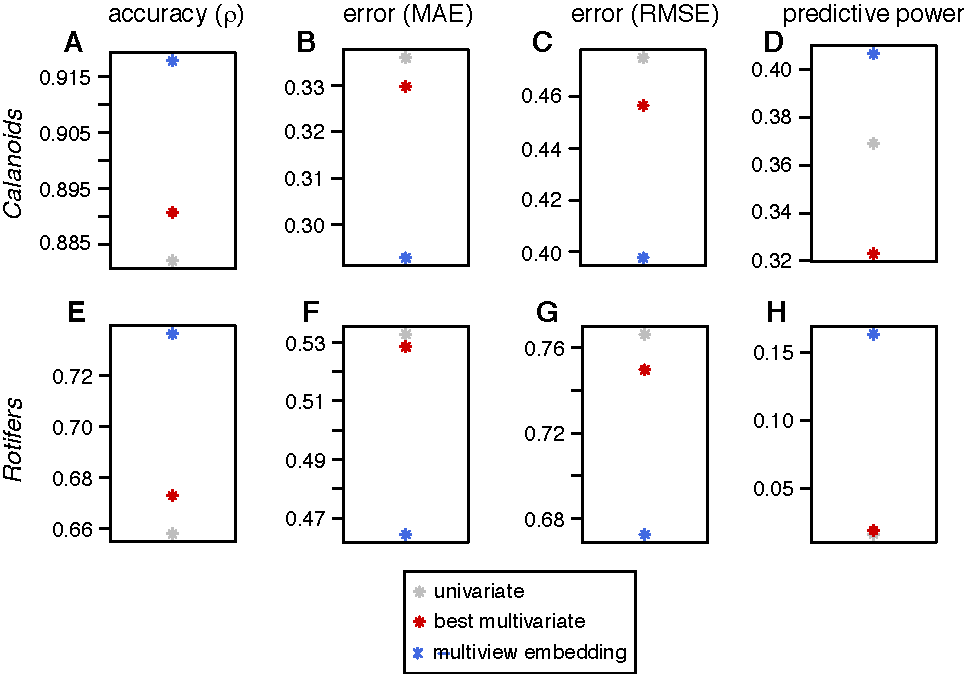
\includegraphics[width=\textwidth]{fig_multiembed_ed_4.pdf}\end{center}
\caption[Comparison of forecast performance for the long-term mesocosm experiment.]{\textbf{Comparison of forecast performance for the long-term mesocosm experiment.}\newline
Multiview embedding produces more precise forecasts than the best multivariate and univariate methods. (A-D) Forecast accuracy ($\rho$, correlation between observations and predictions), forecast errors (MAE, mean absolute error; RMSE, root mean square error), and predictive power when predicting calanoid copepods. (E-H) Forecast accuracy, forecast errors, and predictive power when predicting rotifers.}
\label{fig_multiembed_ed_4}
\end{figure}

\section{Acknowledgments}
This research is supported by Department of Defense, Strategic Environment Research and Development Program W912HQ-15-C-00 (GS, HY), Lenfest Foundation Award 00028335 (GS), National Science Foundation Grant No. DEB-1020372 (GS, HY), NSF-NOAA Comparative Analysis of Marine Ecosystem Organization (CAMEO) program Grant NA08OAR4320894/CAMEO (GS), McQuown Natural Science Research and Education Fund F-2619 (HY), National Science Foundation Graduate Research Fellowships (HY), the Sugihara Family Trust (GS), the Deutsche Bank-Jameson Complexity Studies Fund (GS), and the McQuown Chair in Natural Science (GS).

Chapter \ref{chap_multiembed}, in full, is material prepared for submission: Hao Ye and George Sugihara. Complexity is not a curse: leveraging information in interconnected systems. The dissertation author was the primary investigator and author of this paper.